\documentclass[11pt]{article}
\usepackage[a4paper,margin=2cm]{geometry}
\usepackage{amsmath,amssymb,booktabs,xcolor,enumitem,colortbl,tabularx,array}
\newcolumntype{L}{>{\raggedright\arraybackslash}X}
\usepackage{tikz}
\usetikzlibrary{arrows.meta,positioning,calc}
\usepackage[hidelinks]{hyperref}
\setlist{nosep,leftmargin=1.4em}

\definecolor{arc}{HTML}{1F5FAD}
\definecolor{good}{HTML}{2E7D32}
\definecolor{bad}{HTML}{B3261E}
\definecolor{mid}{HTML}{D9730D}
\definecolor{soft}{HTML}{F2F2F2}
\newcommand{\pend}{\textcolor{gray}{\emph{pending}}}
\newcommand{\gapgood}[1]{\textcolor{good}{\textbf{#1}}}
\newcommand{\gapmid}[1]{\textcolor{mid}{\textbf{#1}}}
\newcommand{\gapbad}[1]{\textcolor{bad}{\textbf{#1}}}
\tikzset{
  box/.style={draw,thick,rounded corners=3pt,align=center,minimum height=11mm,inner sep=4pt,font=\small},
  q/.style={box,fill=arc!10,draw=arc},
  c/.style={box,fill=soft},
  flow/.style={-{Stealth[length=2.6mm]},thick},
  nd/.style={circle,draw,thick,minimum size=6.5mm,inner sep=0pt,fill=white,font=\small},
  ar/.style={-{Stealth[length=2.4mm]},thick,arc},
}

\title{\textbf{Quantum approaches to QOBLIB network design}\\[2pt]
\large Status report: pipeline, configurations explored, and quality vs.\ best known}
\date{21 November 2026}
\author{}

\begin{document}
\sloppy
\maketitle
\vspace{-1cm}

%===========================================================================
\section*{Bottom line}
The score is QOBLIB's official objective (maximum link load, from the exact routing LP).
\emph{Gap} = (our score $-$ best known) / best known: \textbf{lower is better, and 0\% matches
QOBLIB}. \texttt{network05} is proven optimal; \texttt{network12} and \texttt{network24} have best-known values.

\begin{center}
\renewcommand{\arraystretch}{1.25}\small
\begin{tabularx}{\textwidth}{@{}>{\raggedright\arraybackslash}p{24mm}Lrr>{\raggedright\arraybackslash}p{30mm}@{}}
\toprule
instance & best result and method & score & gap & quantum used?\\
\midrule
\texttt{network05} (20 vars) & warm-started QAOA (notebook 00) + polish & 65\,500 & \gapgood{0.00\%} & \textbf{yes}: 20 qubits, 3/3 seeds\\
\texttt{network12} (132 vars) & SA on QUBO + 2-exchange polish & 282\,819 & \gapmid{+2.3\%} & no (classical)\\
\texttt{network12} & best \emph{quantum} pipeline (exchange-mixer local search) & 324\,834 & \gapbad{+17.5\%} & yes: $\le$16 qubits, short run\\
\texttt{network12} & any QUBO sampler alone (incl.\ partitioned QAOA, PCE) & 313\,778 & \gapbad{+13.5\%} & yes / no\\
\texttt{network24} (552 vars) & team submission: parallel tempering + ILS & 657\,121 & \gapgood{$-$0.99\%} & no (classical)\\
\texttt{network24} & quantum pipeline & -- & not run & --\\
\bottomrule
\end{tabularx}
\end{center}

\noindent\textbf{In one sentence:} quantum methods reach the optimum on the smallest instance
(\texttt{network05}, warm-started QAOA), but on \texttt{network12} they are still
13--18\% above best known. Classical search gets within 2.3\% on \texttt{network12} and
beats the best known value on \texttt{network24}.

%===========================================================================
\section{The problem in one paragraph}
Choose a directed network on $n$ nodes in which every node has exactly 2 outgoing and 2 incoming
links. There is one binary variable per possible link, so $n(n-1)$ variables. All traffic is
routed, and the score is the load on the busiest link. A linear program (LP) computes that score
exactly for a given network, so the quantum (or classical) solver only has to \emph{propose
networks}, and the LP judges them.

%===========================================================================
\section{The pipeline}
\begin{center}
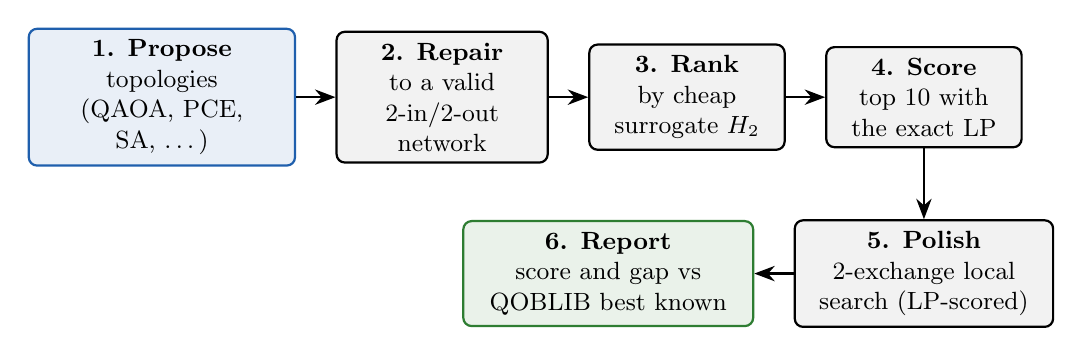
\begin{tikzpicture}[node distance=4mm and 5mm]
  \node[q,text width=31mm] (prop) {\textbf{1. Propose}\\topologies\\(QAOA, PCE, SA, \dots)};
  \node[c,right=of prop,text width=24mm] (rep) {\textbf{2. Repair}\\to a valid\\2-in/2-out network};
  \node[c,right=of rep,text width=22mm] (rank) {\textbf{3. Rank}\\by cheap\\surrogate $H_2$};
  \node[c,right=of rank,text width=22mm] (lp) {\textbf{4. Score}\\top 10 with\\the exact LP};
  \node[c,below=9mm of lp,text width=30mm] (pol) {\textbf{5. Polish}\\2-exchange local\\search (LP-scored)};
  \node[box,fill=good!10,draw=good,left=of pol,text width=34mm] (out) {\textbf{6. Report}\\score and gap vs\\QOBLIB best known};
  \draw[flow] (prop)--(rep); \draw[flow] (rep)--(rank); \draw[flow] (rank)--(lp);
  \draw[flow] (lp)--(pol); \draw[flow] (pol)--(out);
\end{tikzpicture}
\end{center}
\noindent\textcolor{arc}{\textbf{Blue}} = quantum step. Every configuration goes through the
\emph{same} steps 2--6 and is compared with a \emph{polish-only} baseline (random start, same LP
budget), which shows whether the quantum step adds anything.

\paragraph{Key terms.}
\begin{itemize}
\item \textbf{Valid topology}: every node has exactly 2 out-links and 2 in-links. Almost no
  bitstrings are valid: about $5\cdot10^{-25}$ of them for \texttt{network12}.
\item \textbf{2-exchange}: the smallest legal change, $(a\!\to\!b),(c\!\to\!d)\Rightarrow
  (a\!\to\!d),(c\!\to\!b)$. It changes 4 bits at once and keeps the network valid.
\item \textbf{$H_2$ surrogate}: total traffic $\times$ hops, with hops capped at 3. It is cheap to compute and
  well correlated with the LP score (Spearman 0.85 near good solutions on \texttt{network12}).
\end{itemize}

\paragraph{Where jobs run.}
\begin{center}\small
\begin{tabularx}{\textwidth}{@{}llL@{}}
\toprule
job size & backend & notes\\
\midrule
$<$25 qubits, $<$4 min & local Maestro simulator & free\\
$<$25 qubits, longer & Qoro cloud \texttt{qoro\_cpu} & about 1 credit per job\\
$\ge$25 qubits & Qoro cloud \texttt{qoro\_gpu} & one-batch cost probe first; 30 qubits cost 515 credits per batch\\
\bottomrule
\end{tabularx}
\end{center}

%===========================================================================
\section{What we explored}
\renewcommand{\arraystretch}{1.15}
\begin{center}\small
\begin{tabularx}{\textwidth}{@{}>{\raggedright\arraybackslash}p{27mm}L>{\raggedright\arraybackslash}p{42mm}>{\raggedright\arraybackslash}p{24mm}@{}}
\toprule
step / family & configurations (knobs) & outcome & verdict\\
\midrule
\multicolumn{4}{@{}l}{\textbf{A. How the objective is written (QUBO formulation)}}\\
direct-link QUBO & notebook 02: reward links that carry direct demand; degree rules as a penalty with weight $\lambda$ & ranks networks poorly (Spearman 0.07--0.71) & baseline\\
path-variable QUBO & extra variables for 2-hop (and 3-hop) paths; strict and soft penalty forms & much better ranking (0.32--0.91), but 8$\times$ more variables & \textcolor{mid}{accurate but unsolvable}\\
exact $H_2$ HUBO & degree-4 polynomial, exact on valid networks, no penalties & used with the exchange mixer & \textcolor{good}{works}\\
node-load L2 & penalise $(S_j+\text{transit}_j)^2$, i.e.\ route traffic via quiet nodes & best ranking of all (0.85 / 0.95 near) & \textcolor{good}{promising}\\
\midrule
\multicolumn{4}{@{}l}{\textbf{B. How topologies are proposed (step 1)}}\\
SA / tabu on QUBO & 2k--20k sweeps, $\lambda=1\ldots6$ & stuck above good energies & classical baseline\\
QAOA, X mixer & layers 2/4/6, $\lambda$ 0.5/2, blind vs.\ warm start & warm start: 100\% valid, optimum on \texttt{network05} & \textcolor{good}{best quantum}\\
QAOA, exchange mixer & layers 1--4; full problem, or local search on 4 freed links & always 100\% valid; blind angles weak & \textcolor{mid}{valid, needs tuning}\\
PCE & Dense / Poly encoding, alpha 2/4 & 0/100 valid on \texttt{network12} & \textcolor{bad}{parked}\\
partitioned QAOA / PCE & cluster size 8/12/16, modularity / spectral & partitions break the degree rules: 0--15\% valid & \textcolor{bad}{parked}\\
\midrule
\multicolumn{4}{@{}l}{\textbf{C. Post-processing (steps 2--5)}}\\
single-bit local search & Divi's default \texttt{local\_search} & cannot repair the degree rules & replaced\\
2-exchange polish & rank neighbours by $H_2$, LP-score the top 5 & $+$10\% $\to$ $+$2.3\% on \texttt{network12} & \textcolor{good}{essential}\\
\bottomrule
\end{tabularx}
\end{center}

%===========================================================================
\section{Results on \texttt{network05} (proven optimum 65\,500)}
Configuration sweep on the local simulator, with 3 random seeds per configuration. Each run may use
only its first 20 samples, then 10 LP scores and 20 polish steps (30 LP evaluations in total). The
\textbf{polish-only baseline}, with the same 30 LP evaluations, hits the optimum on \textbf{1/3} seeds.

\begin{center}\small
\begin{tabularx}{\textwidth}{@{}Lccccr@{}}
\toprule
configuration & valid & opt.\ sampled & opt.\ after polish & mean gap & time\\
\midrule
\rowcolor{good!10}
\textbf{QAOA X mixer, 6 layers, warm start} & \textbf{100\%} & \textbf{3/3} & \textbf{3/3} & \textbf{0.0\%} & 31 s\\
QAOA X mixer, 2 layers, $\lambda=2$ & 0\% & 2/3 & 3/3 & 0.0\% & 13 s\\
QAOA X mixer, 2 layers, $\lambda=0.5$ & 20\% & 1/3 & 2/3 & 1.3\% & 18 s\\
QAOA X mixer, 4 layers, $\lambda=0.5$ & 0\% & 1/3 & 2/3 & 1.3\% & 22 s\\
QAOA X mixer, 4 layers, $\lambda=2$ & 7\% & 1/3 & 2/3 & 1.3\% & 22 s\\
QAOA exchange mixer, 2 layers (blind) & 100\% & 0/3 & 1/3 & 2.5\% & 270 s\\
QAOA exchange mixer, 3 layers (blind) & 100\% & 0/3 & 0/3 & 5.5\% & 400 s\\
\midrule
exchange mixer 4 layers; PCE (4); partitioned (3) & \multicolumn{5}{c}{\pend\ (sweep still running)}\\
\bottomrule
\end{tabularx}
\end{center}
\noindent\textbf{Reading:} the warm start from Divi's \texttt{characterize\_and\_validate}
(notebook 00) is the only configuration that finds the optimum \emph{directly} on every seed.
Blind QAOA and the exchange mixer reach it only through the classical polish, about as often as
the baseline does. With only 216 valid networks, \texttt{network05} is easy: it is a test
bed, not evidence that the method scales.

%===========================================================================
\section{Results on \texttt{network12} (best known 276\,474)}
\begin{center}\small
\begin{tabularx}{\textwidth}{@{}L>{\raggedright\arraybackslash}p{30mm}rr@{}}
\toprule
method & quantum step & best score & gap\\
\midrule
any QUBO sampler alone (SA, tabu, partitioned QAOA, PCE) & some & 313\,778 & \gapbad{+13.5\%}\\
quantum local search, exchange mixer, 15 steps (2 seeds) & QAOA, $\le$16 qubits & 324\,834 & \gapbad{+17.5\%}\\
\quad same budget: random proposals & -- & 336\,334 & +21.7\%\\
\quad same budget: classical $H_2$ ranking & -- & 332\,905 & +20.4\%\\
classical local search, 40 steps + polish & -- & 291\,667 & \gapmid{+5.5\%}\\
\textbf{SA on QUBO + 2-exchange polish} & -- & \textbf{282\,819} & \gapmid{\textbf{+2.3\%}}\\
\bottomrule
\end{tabularx}
\end{center}
The quantum local search beat random and classical proposers at equal budget on both seeds. But
the runs were short (15 steps), and the 40-step quantum run was cancelled by the Qoro scheduler, so
there is no converged quantum result on \texttt{network12} yet.

%===========================================================================
\section{Main lessons}
\begin{enumerate}
\item \textbf{Penalties are the main obstacle.} Two valid networks are at least 4 bit flips apart,
  and each intermediate state pays a penalty of $2\lambda$. Samplers that flip single bits (SA,
  X-mixer QAOA, partitioning, PCE rounding) rarely land on valid networks. \emph{Fixes:} move by
  2-exchanges (the polish), or use the \textbf{exchange mixer}, a QAOA mixer whose every state is a
  valid network. This was verified exactly: the probability of a valid network stays at 1.
\item \textbf{Warm starts matter more than depth.} Notebook 00's warm start (angles from
  \texttt{characterize\_and\_validate}, 10 credits) beat every blind configuration on \texttt{network05}.
\item \textbf{The cost function is not the bottleneck on small instances.} On \texttt{network05} the
  LP optimum is the ground state of $H_2$; without a good start, QAOA simply does not concentrate on it.
\item \textbf{Full-problem QAOA does not scale on simulators.} 30 qubits cost 515 credits for one
  optimiser batch, with no result; 42 qubits failed outright. Scaling has to go through
  sub-problems of 16--20 qubits or fewer, such as the quantum local search.
\item \textbf{Classical post-processing carries the score.} The 2-exchange polish is worth 7--10
  percentage points on \texttt{network12}, more than any quantum change so far.
\end{enumerate}

\section{Next steps}
\begin{enumerate}
\item Finish the \texttt{network05} sweep, then confirm the top configurations with 5 seeds
  (\texttt{qoro\_cpu}, at most 300 credits).
\item Warm-start the exchange mixer too (angles from the service or from smaller instances).
\item Run the quantum local search on \texttt{network12} to convergence, with warm starts and the
  node-load L2 cost, and report its gap vs best known.
\item \textbf{Parked:} PCE and partitioned QAOA, which break the degree rules. Revisit them with
  constraint-aware partitions or valid-repair decoding.
\end{enumerate}

%===========================================================================
\appendix
\section{Appendix: the two quantum ingredients}
\paragraph{Exact $H_2$ cost (HUBO).} With $\tau_{ik}$ the normalised demand and $p_j=x_{ij}x_{jk}$
(path $i\to j\to k$ exists), on valid networks
\[
  H_2=\sum_{i\neq k}\tau_{ik}\Big[3-2x_{ik}-\sum_j p_j+\sum_{j<j'}p_jp_{j'}+x_{ik}\sum_j p_j\Big].
\]
This is exact because each node has only 2 out-links. It has degree 4, no penalties and no extra variables.

\paragraph{Exchange mixer.} One term per 2-exchange $q=(ab,cd\to ad,cb)$:
$M_q=\sigma^-_{ab}\sigma^-_{cd}\sigma^+_{ad}\sigma^+_{cb}+\text{h.c.}$, which is 8 commuting Pauli strings.
\begin{center}
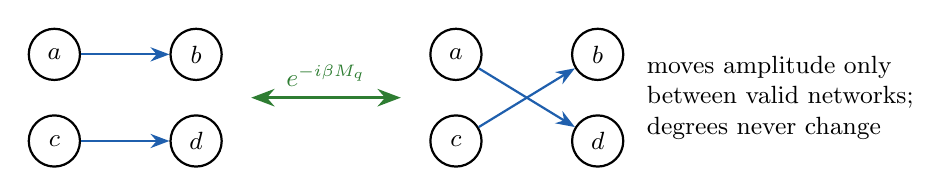
\begin{tikzpicture}
  \begin{scope}
    \node[nd] (a) at (0,1.1) {$a$}; \node[nd] (b) at (1.8,1.1) {$b$};
    \node[nd] (c) at (0,0) {$c$};   \node[nd] (d) at (1.8,0) {$d$};
    \draw[ar] (a)--(b); \draw[ar] (c)--(d);
  \end{scope}
  \draw[{Stealth}-{Stealth},very thick,good] (2.5,0.55) -- node[above,font=\small]{$e^{-i\beta M_q}$} (4.4,0.55);
  \begin{scope}[xshift=5.1cm]
    \node[nd] (a) at (0,1.1) {$a$}; \node[nd] (b) at (1.8,1.1) {$b$};
    \node[nd] (c) at (0,0) {$c$};   \node[nd] (d) at (1.8,0) {$d$};
    \draw[ar] (a)--(d); \draw[ar] (c)--(b);
  \end{scope}
  \node[font=\small,align=left,anchor=west] at (7.4,0.55) {moves amplitude only\\between valid networks;\\degrees never change};
\end{tikzpicture}
\end{center}

\vfill\noindent\footnotesize
Code: \texttt{network\_sweep.py} (configuration sweep), \texttt{network\_mixer.py} (exchange mixer,
quantum local search), \texttt{network\_moves.py} (2-exchange polish, surrogates),
\texttt{network\_hopqubo*.py} (path-variable QUBOs). Logs are in \texttt{runs/}; team submissions are in
\texttt{deliverables/}.
\end{document}
